\documentclass{beamer}

\usepackage{latexsym,graphicx}
\usepackage{pgf,tikz}
\usepackage{amsmath,amssymb}
\usepackage{amsthm}
\usepackage{enumerate}
\usepackage{graphicx}
\usepackage{hyperref}
\usepackage{url}
\usepackage{framed}
\usepackage{cleveref}
\usepackage{comment}
\usepackage{color}
\usetikzlibrary{arrows}
\usepackage[]{algorithm2e}
\usepackage{framed}
\usepackage{subcaption}
\captionsetup{compatibility=false}


\setbeamertemplate{navigation symbols}{}

%%% TEMPLATE PARAMETERS %%%

%%% TITLE %%%
  
% Useful macros
\newcommand{\E}[1]{\mathbf{E}\l[#1\r]}
\renewcommand{\l}{\left}
\renewcommand{\r}{\right}
\renewcommand{\iff}{\Leftrightarrow}
\newcommand{\intff}{\int_{-\infty}^\infty }
\newcommand{\intzf}{\int_0^\infty }
\newcommand{\intpp}{\int_{-\pi}^\pi }
\newcommand{\sumzf}[1]{\sum_{#1=0}^\infty}
\newcommand{\sumff}[1]{\sum_{#1=-\infty}^\infty}
\newcommand{\Bin}{\text{Bin}}
\newcommand{\pfrac}[2]{\l(\frac{#1}{#2}\r)}
\renewcommand{\bf}{\textbf}
\newcommand{\zm}[1]{z^{-#1}}
\renewcommand{\P}[1]{\mathbf{P}\l\{#1\r\}}
\newcommand{\Var}[1]{\mathbf{Var}\l(#1\r)}
\newcommand{\Poiss}{\text{Poiss}}
\newcommand{\Geom}{\text{Geom}}
\newcommand{\Skew}{\text{\bf{Skew}}}
\newcommand{\minimize}{\text{minimize }}
\newcommand{\subjectTo}{\text{subject to }}

\newtheorem{claim}{Claim}
\newtheorem{assumption}{Assumption}
\newtheorem{challenge}{Challenge}
\newtheorem{observation}{Observation}
\newtheorem{openproblem}{Open Problem}
\newtheorem{openquestion}{Open question}


\newcommand{\todo}[1]{\noindent {\color{red} {  \bf \large TODO:} #1}}
\newcommand{\beq}{\begin{equation}}
\newcommand{\eeq}{\end{equation}}
\newcommand{\beas}{\begin{eqnarray*}}
\newcommand{\eeas}{\end{eqnarray*}}

\newcommand{\poly}{\mathrm{poly}}
\newcommand{\eps}{\epsilon}
\newcommand{\e}{\epsilon}
\newcommand{\polylog}{\mathrm{polylog}}
\newcommand{\rob}[1]{\left( #1 \right)} %Round Brackets
\newcommand{\sqb}[1]{\left[ #1 \right]} %square Brackets
\newcommand{\cub}[1]{\left\{ #1 \right\} } %curly brackets
\newcommand{\rb}[1]{\left( #1 \right)} %Round
\newcommand{\abs}[1]{\left| #1 \right|} %| |
\newcommand{\zo}{\{0, 1\}}
\newcommand{\zonzo}{\zo^n \to \zo}
\newcommand{\zokzo}{\zo^k \to \zo}
\newcommand{\zot}{\{0,1,2\}}
\newcommand{\norm}[1]{\left\lVert#1\right\rVert}
%
%\newcommand{\en}[1]{\marginpar{\textbf{#1}}}
%\newcommand{\efn}[1]{\footnote{\textbf{#1}}}
\newcommand{\bR}{\mathbb{R}}
\newcommand{\bE}{\mathbb{E}}
\DeclareMathOperator*{\argmin}{arg\,min}
\DeclareMathOperator*{\argmax}{arg\,max}

\newcommand{\bN}{\mathbb{N}}
\newcommand{\Greedy}{\textsc{Greedy }}
\newcommand{\OPT}{\textsc{Opt }}
\newcommand{\benef}{\text{benef}}

\newtheorem*{outputt}{Output}
\newtheorem*{goall}{Goal}
\newtheorem*{inputt}{Input}
\newtheorem{assump}{Assumption}

\usetheme{Pittsburgh}
\usecolortheme{beaver}

\title{NOOC Paper Review\\Gossip vs. Markov Chains}
\author{Jean-Baptiste Cordonnier and Ismail Bouanani}
\date{\today}

\begin{document}

% \AtBeginSection[]
% {
%  \begin{frame}<beamer>
%  \frametitle{Plan}
%  \tableofcontents[currentsection]
%  \end{frame}
% }

%%%%%% PLAN FRAME %%%%%

 % \begin{frame}<beamer>
 % \frametitle{Plan}
 % \tableofcontents[currentsection]
 % \end{frame}

\frame{\titlepage}

\begin{frame}{Overview}
\tableofcontents
\end{frame}


\section {Proof outline}

\frame{\sectionpage}

  \begin{frame}
  \begin{itemize}

    \frametitle{ Approximation via Random walks}
    
    \item The problem of rumor spreading is comparable to multiple parallel random walks.
   \item    If node u informs  v, a random walk goes from $u$ to $v$ $(S_i = \overline{lazy}$), another one remains at $u$ $(S_i=lazy)$. 
   \begin{figure}[h]
\centering
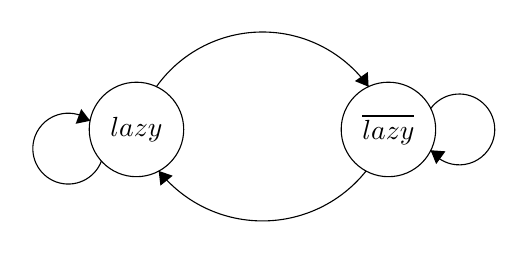
\begin{tikzpicture}[scale=0.2]
\tikzstyle{every node}+=[inner sep=0pt]
\draw [black] (26.1,-26.6) circle (3);
\draw (26.1,-26.6) node {$lazy$};
\draw [black] (42.1,-26.6) circle (3);
\draw (42.1,-26.6) node {$\overline{lazy}$};
\draw [black] (40.688,-29.229) arc (-38.4609:-141.5391:8.413);
\fill [black] (27.51,-29.23) -- (27.62,-30.17) -- (28.4,-29.54);
\draw [black] (27.358,-23.895) arc (144.65362:35.34638:8.265);
\fill [black] (40.84,-23.89) -- (40.79,-22.95) -- (39.97,-23.53);
\draw [black] (23.878,-28.598) arc (-20.31276:-308.31276:2.25);
\fill [black] (23.16,-26.05) -- (22.59,-25.3) -- (22.24,-26.24);
\draw [black] (44.78,-25.277) arc (144:-144:2.25);
\fill [black] (44.78,-27.92) -- (45.13,-28.8) -- (45.72,-27.99);
\end{tikzpicture}

\label{fig:lazyFSM}
\end{figure}

\end{itemize}

  \end{frame}
\begin{frame}
\begin{itemize}
\frametitle{Forward and reversed random walks}
\item Rumor sharing is dual : if $u$ pushes to $v$, $v$ pulls from $u$
\item 2 types of random walks: forward (pushing from a source) and reversed (pulling from a target). 
\item If a forward random walk takes a step from $u$ to $v$, a reversed one   takes a step form $v$ to $u$, if $u$ is the only node pushing to $v$.
\item Reversed random walks are only an analytic tool (no pull in practice)
 
\end{itemize}

\end{frame}


\begin{frame}
\begin{itemize}
\frametitle{Probabilistic computations}
\item Node $w$ is reached by the information within $k$ rounds if there is $k/2$ steps forward (from source $s$) and $k/2$ steps backward (from $w$) that meet at a certain node.
\item  Union bound over all the transiting nodes and all the possible patterns $\{ lazy,\overline{lazy} \}^k$
\begin{align*}
  \scriptsize
  P\l(w \text{ informed in T rounds}\r) \geq P\l(\sum_{S,S'\in \mathcal C_{T/2}, u\in V[G]} X_{s,u}^S Y_{w,u}^{S'} > 0\r)
\end{align*}
 where $X_{s,u}^S$ and $Y_{w,u}^{S'}$ are indicator random variables on the existence of such walks

\end{itemize}


\end{frame}

\begin{frame}
\begin{itemize}
\frametitle{Notations}
\item We analyze random walks pair wisely with Markov Chains coupling. It's a way to represent their joint evolution
\item We use the lazy matrix $
  \mathcal L _ \gamma (\mathbf{M}) \triangleq (1-\gamma) \mathbf{I} + \gamma \mathbf{M}
$

  (\textbf{M} with self-edge eventuality)
\item Doeblin coupling  : once two walks meet at the same node $u$, they are never separated again.
\[
  \mathcal Q(\mathbf{M})_{(u,w)(v,x)} \triangleq \left\{
    \begin{array}{ll}
      (\mathbf{M} \otimes \mathbf{M})_{(u,w)(v,x)} & u \not = v,\\
      \mathbf{M}_{(u,v)} \cdot \mathbf{1}_{v = x} & u = v.\\
    \end{array}
  \right.
\]


\end{itemize}
\end{frame}




\begin{frame}{Stationary distribution}
\begin{itemize}


 \item Show a bound on the stationary distribution after $k$ steps, $\to \pi \otimes \pi$

\item Upper bound:
\[
  \norm{u(\mathcal L_{\gamma,\gamma} \circ \mathcal Q(M))^k - \pi \otimes \pi}_2 \leq (1 - \gamma \alpha / 2)^k + 2 \sqrt 2 \gamma \alpha^{-1} n^{-3/2}
\]
with $u$ being a distribution over V[G] x V[G] and $\gamma = \min(1/3, \Delta^{0.5-c}\alpha/9)$

\item Right side goes to 0 under certain condition

\item Once the Markov chain mixes, all nodes have been informed

\end{itemize}
\end{frame}


\section{Intuition}

\frame{\sectionpage}

\begin{frame}{Intuition}
  \begin{itemize}
    \item What is a "good" / "bad" graph ? 

    \item Captured by the parameter $\alpha$ and the regularity $\beta$
    \begin{itemize}
      \item $\beta = \Delta / \delta$
      \item $\alpha = 1 - \lambda_2$ where $\lambda_2$ is the second highest eigenvalue of the normalized adjacency matrix
      \item $\alpha$ is strongly related to the conductance of the graph $G$ (Cheeger's Innequality)
    \end{itemize}

    \item Conductance of a graph
      \[
        \Phi(G) \triangleq \min_{\emptyset \not = S \subset V} \frac{e(S, V \setminus S)}{\min(\text{vol}(S), \text{vol}(V \setminus S))}
      \]
  \end{itemize}
\end{frame}

\begin{frame}{Conductance}
      \[
        \Phi(G) \triangleq \min_{\emptyset \not = S \subset V} \frac{e(S, V \setminus S)}{\min(\text{vol}(S), \text{vol}(V \setminus S))}
      \]
      \begin{center}
        
  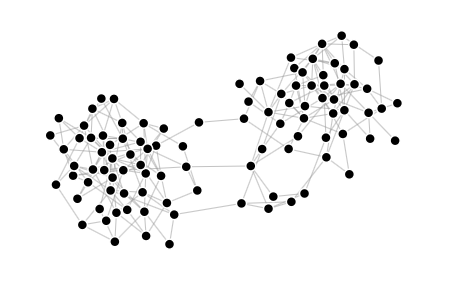
\includegraphics[width=.9\linewidth]{graph}
      \end{center}
\end{frame}


\section{Simulation}

\frame{\sectionpage}

\begin{frame}{Simulations Set Up}
\begin{itemize}
  \item 
    First simple model of random graphs $C(n,p)$

  \item
    More realistic model of real world network: Barabasi-Albert
  \item More interesting to study "weird" graphs (with bottle neck for instance): 
  \begin{itemize}
    \item two independent graphs $G_1, G_2 \sim C(n,p)$
    \item edges $G_1 \leftrightarrow G_2$ with probability $q \ll p$all
  \end{itemize}
\end{itemize}

\end{frame}

\begin{frame}{Simulation}
  
\end{frame}

\begin{frame}{Results}
  \begin{table}
\centering
\begin{tabular}{c|c|c||c|c|c}
  $q (10^{-5})$ & \# crossing & $\alpha (10^{-4})$ & .5 & .9 & 1\\
  \hline
  1 & 8 & 1.5 & 13 & 21 & 22 \\
1.3 & 15 & 2.9 & 13 & 20 & 21 \\
1.7 & 28 & 5.5 & 13 & 19 & 20 \\
2.2 & 18 & 3.5 & 13 & 20 & 21 \\
2.8 & 33 & 6.4 & 13 & 19 & 20 \\
3.6 & 43 & 8.4 & 13 & 18 & 20 \\
4.6 & 51 & 10.0 & 13 & 18 & 20 \\
6.0 & 57 & 11.2 & 13 & 18 & 19 \\
7.7 & 73 & 14.2 & 13 & 18 & 19 \\
10 & 129 & 25.2 & 13 & 17 & 18 \\
\end{tabular}
\caption{Quantiles of informed node during rumor spreading protocol on a bottle neck graph with bridging probability $q$, $n = 2 \cdot 1000$ and $p = 0.1$}
\label{tab:quantiles}
\end{table}
\end{frame}

\begin{frame}{Conclusion}

\begin{itemize}
  \item Very strong result: $O(\log n)$ bound for any graph
  \item Applicable to wide range of graphs, minimal assumptions
  \item Not representative of social networks
  \begin{itemize}
    \item uniform choice instead of distance/weight related choice
    \item Does not apply to sharing the gossip with a group
  \end{itemize}
  \item Implementation boils down to finding a good way to pick a random neighbor (hot topic)
  \item Sacrifice some performance to need less entropy
\end{itemize}
  
\end{frame}

\begin{frame}
  
\end{frame}

\begin{frame}{Appendix}
  \begin{center}
    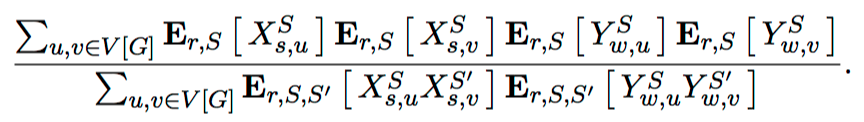
\includegraphics[width=1\linewidth]{lower_bound_exp.png}
  \end{center}
\end{frame}

\end{document}
